\documentclass[tikz,border=1pt,11pt]{standalone}
% Shared style for all diagrams. Text: Times; mathematics: Computer Modern, as in the paper.
% Figures are drawn at the paper's text width (432pt = 15.24cm), so sizes below are final.
\usepackage[T1]{fontenc}
\usepackage{times}
\usepackage{amsmath,amssymb}
\usepackage{pgfplots}
\usetikzlibrary{arrows.meta,calc,positioning,backgrounds,patterns,shapes.geometric}
\usepgfplotslibrary{groupplots,fillbetween}
\pgfplotsset{compat=1.18}
% Palette. Three identity hues (validated with the dataviz colour checks: lightness band,
% chroma floor, all-pairs CVD separation >= 8.9, normal-vision separation >= 18.5,
% contrast >= 3:1 on white) plus neutral inks and pale region fills.
\definecolor{ink}{HTML}{1D2733}      % text and exact reference curves
\definecolor{muted}{HTML}{56606B}    % secondary text
\definecolor{rule}{HTML}{8A929A}     % axes, guides
\definecolor{assess}{HTML}{1F6FA8}   % assessments; stable branches
\definecolor{process}{HTML}{1E9E73}  % accumulated processing
\definecolor{event}{HTML}{C5531F}    % completions, resets, driven paths
\definecolor{tolfill}{HTML}{E3EDF5}  % tolerance region
\definecolor{transfill}{HTML}{F2F4F6}% transition region
\definecolor{pausefill}{HTML}{E4F3EC}% processing paused
\tikzset{
 >={Stealth[length=2.1mm,width=1.5mm]},
 every picture/.append style={font=\small},
 lbl/.style={font=\small,text=ink,inner sep=1.5pt},
 note/.style={font=\footnotesize,text=muted,inner sep=1.5pt},
 paneltitle/.style={font=\small\bfseries,text=ink,inner sep=0pt},
 guide/.style={rule,line width=.45pt,densely dotted},
 report/.style={diamond,draw=ink,fill=white,line width=.8pt,inner sep=0pt,minimum size=5.2pt},
}
\pgfplotsset{
 every axis/.append style={
  axis lines*=left,
  axis line style={rule,line width=.5pt},
  tick style={rule,line width=.5pt},
  major tick length=2.2pt,
  tick align=outside,
  label style={font=\small,text=ink},
  tick label style={font=\small,text=ink},
  every axis plot/.append style={line width=1.15pt},
  scaled ticks=false,
  clip=false,
  xlabel style={inner sep=1pt},
  ylabel style={inner sep=1pt},
 },
}

% Figure 3. Killing and reinjection in the forward equation (schematic, not computed).
% A: the stationary density of assessments, with the tolerance band; outside it processing has
% accumulated and completions concentrate. B: completions remove that mass and reinject it at the
% reset level (capped reset, theta/2). C: just after, tails thinner and mass at the reset level.
% D: drift, diffusion and reinjection balance in the stationary law; a small common push acts on it
% through the direction -d pi/du, and feedback through the average adds a rank-one term.
\begin{document}
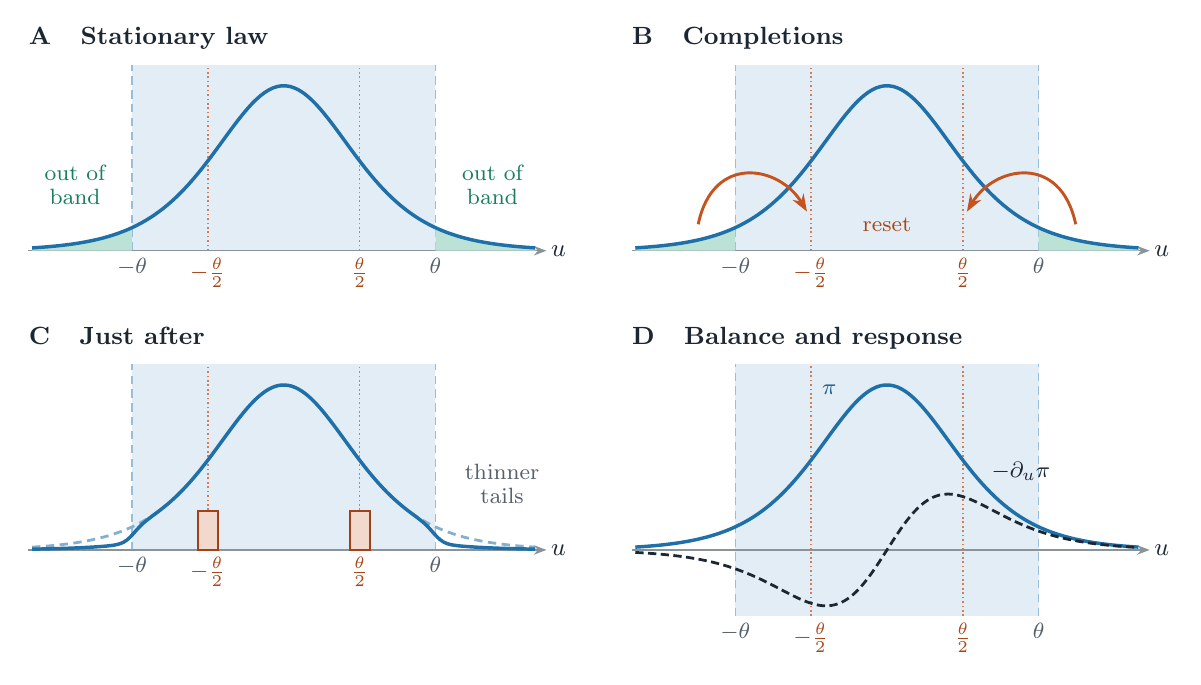
\begin{tikzpicture}[x=0.94cm,y=0.80cm]
\def\Th{2.05}
\def\Tg{1.025}
% stationary density (schematic): pi(u) = 2.62 sech^2(u/1.25)
\def\dens(#1){2.62/(cosh((#1)/1.25))^2}
\tikzset{
 dens/.style={assess,line width=1.25pt},
 olddens/.style={assess!55,line width=1.0pt,densely dashed},
 resp/.style={ink,line width=1.0pt,dash pattern=on 3pt off 1.6pt},
 move/.style={event,line width=1.05pt,-{Stealth[length=2.2mm,width=1.6mm]}},
}
% one panel: title, lowest level of the band (below the axis when a signed curve is drawn)
\newcommand{\Frame}[2]{%
  \fill[tolfill] (-\Th,#2) rectangle (\Th,2.95);
  \draw[assess!45,line width=.4pt,densely dashed] (-\Th,#2) -- (-\Th,2.95);
  \draw[assess!45,line width=.4pt,densely dashed] (\Th,#2) -- (\Th,2.95);
  \draw[event!75,line width=.6pt,densely dotted] (-\Tg,#2) -- (-\Tg,2.95);
  \draw[event!75,line width=.6pt,densely dotted] (\Tg,#2) -- (\Tg,2.95);
  \draw[rule,line width=.5pt,-{Stealth[length=1.6mm,width=1.2mm]}] (-3.45,0) -- (3.55,0);
  \node[lbl,anchor=west] at (3.55,0) {$u$};
  \foreach \x/\t in {-2.05/{$-\theta$},2.05/{$\theta$}}{\node[note,anchor=north] at (\x,{#2-0.04}) {\t};}
  \foreach \x/\t in {-1.025/{$-\tfrac{\theta}{2}$},1.025/{$\tfrac{\theta}{2}$}}{\node[note,text=event!85!black,anchor=north] at (\x,{#2-0.04}) {\t};}
  \node[paneltitle,anchor=north west] at (-3.45,3.55) {#1};
}
% ---------------------------------------------------------------- (A) stationary law
\begin{scope}[shift={(0,0)}]
\Frame{A\quad Stationary law}{0}
\fill[process!30] (-3.4,0) -- plot[domain=-3.4:-\Th,samples=30] (\x,{\dens(\x)}) -- (-\Th,0) -- cycle;
\fill[process!30] (\Th,0) -- plot[domain=\Th:3.4,samples=30] (\x,{\dens(\x)}) -- (3.4,0) -- cycle;
\draw[dens] plot[domain=-3.4:3.4,samples=120] (\x,{\dens(\x)});
\node[note,text=process!80!black,align=center] at (-2.82,1.05) {out of\\[-1pt]band};
\node[note,text=process!80!black,align=center] at (2.82,1.05) {out of\\[-1pt]band};
\end{scope}
% ---------------------------------------------------------------- (B) completions
\begin{scope}[shift={(8.15,0)}]
\Frame{B\quad Completions}{0}
\fill[process!30] (-3.4,0) -- plot[domain=-3.4:-\Th,samples=30] (\x,{\dens(\x)}) -- (-\Th,0) -- cycle;
\fill[process!30] (\Th,0) -- plot[domain=\Th:3.4,samples=30] (\x,{\dens(\x)}) -- (3.4,0) -- cycle;
\draw[dens] plot[domain=-3.4:3.4,samples=120] (\x,{\dens(\x)});
\draw[move] (-2.55,0.42) .. controls (-2.35,1.55) and (-1.45,1.35) .. (-1.08,0.62);
\draw[move] (2.55,0.42) .. controls (2.35,1.55) and (1.45,1.35) .. (1.08,0.62);
\node[note,text=event!85!black,align=center] at (0,0.42) {reset};
\end{scope}
% ---------------------------------------------------------------- (C) just after
\begin{scope}[shift={(0,-4.75)}]
\Frame{C\quad Just after}{0}
\draw[olddens] plot[domain=-3.4:3.4,samples=120] (\x,{\dens(\x)});
\fill[event!22] (-1.16,0) rectangle (-0.89,0.62);
\fill[event!22] (0.89,0) rectangle (1.16,0.62);
\draw[event!80!black,line width=.7pt] (-1.16,0) rectangle (-0.89,0.62);
\draw[event!80!black,line width=.7pt] (0.89,0) rectangle (1.16,0.62);
\draw[dens] plot[domain=-3.4:3.4,samples=160] (\x,{\dens(\x)*(1-0.72/(1+exp(-min(max((abs(\x)-\Th)/0.07,-8),8))))});
\node[note,align=center] at (2.95,1.05) {thinner\\[-1pt]tails};
\end{scope}
% ---------------------------------------------------------------- (D) balance and response
\begin{scope}[shift={(8.15,-4.75)}]
\Frame{D\quad Balance and response}{-1.05}
\draw[dens] plot[domain=-3.4:3.4,samples=120] (\x,{\dens(\x)});
\draw[resp] plot[domain=-3.4:3.4,samples=160] (\x,{0.55*2.62*1.6*tanh(\x/1.25)/(cosh(\x/1.25))^2});
\node[note,text=ink,anchor=west] at (1.35,1.25) {$-\partial_u\pi$};
\node[note,text=assess!85!black,anchor=east] at (-0.62,2.55) {$\pi$};
\end{scope}
\end{tikzpicture}
\end{document}
